\chapter{Introdução}
\label{chap:intro}
\begin{flushright}
	"O saber que não vem da experiência, não é realmente saber." \\
	\ \\
	(Lev Vygotsky)
\end{flushright}

Quando se ouve falar em robôs, logo associa-se a algo de extrema complexidade. Isso ocorre, sumariamente, devido à falta de informações simplificadas sobre o tema, ou devido a dificuldade de acesso a tais conteúdos. A palavra robótica é derivada da palavra robô, que, segundo \cite{goncalves2007}, é um dispositivo eletromecânico capaz de realizar tarefas de maneira autônoma ou pré-programada, e faz menção a ciência que estuda, cria e aplica robôs. 
No meio educacional, a palavra didática está presente de forma quase que impreterível, afinal, materiais didáticos, livros, projetos e a própria didática como um instrumento qualificador do professor, são componentes fundamentais do cotidiano educacional.

Porém, é notório que barreiras na educação da atualidade estão sendo quebradas. Já se vê espaços de ensino, como por exemplo o citado por \cite{Mataric}, onde o estudante passa a frequentar menos as salas de aula e se engaja mais em projetos, tornando assim o professor apenas um facilitador do aprendizado do aluno, um tutor. A tutoria é um método muito utilizado para efetivar uma interação pedagógica. Um exemplo disso, é que segundo \cite{sa1998}, na educação à distância, o tutor recebe o significado de "orientador de aprendizagem do aluno solitário e isolado".

O sistema de tutoria torna mais fácil o acesso do aluno ao conhecimento, pois o professor passa a ser apenas um orientador, desta maneira o aluno tende a tornar-se independente na busca das informações. Percebendo essa nova dinâmica da educação, e a falta de informações simplificadas sobre robótica, notou-se a possibilidade de criar um kit didático, para incentivar as pessoas através de desafios e simplificar as informações em torno da robótica.

Ultimamente, segundo o resumo executivo World Robotics 2018 Robôs Industriais da International Federation of Robotics\cite{ifr2018}, houve uma crescente utilização de sistemas robóticos e autônomos na nossa sociedade. A demanda global de robôs tem crescido severamente, com estimativa de acréscimo de 14\% ao ano até 2021, como visto na figura~\ref{fig:just_1}.

\begin{figure}[h!]										\caption{Estimativa anual de produção global de robôs até o ano de 2021} \label{fig:just_1}		
	\centering										
	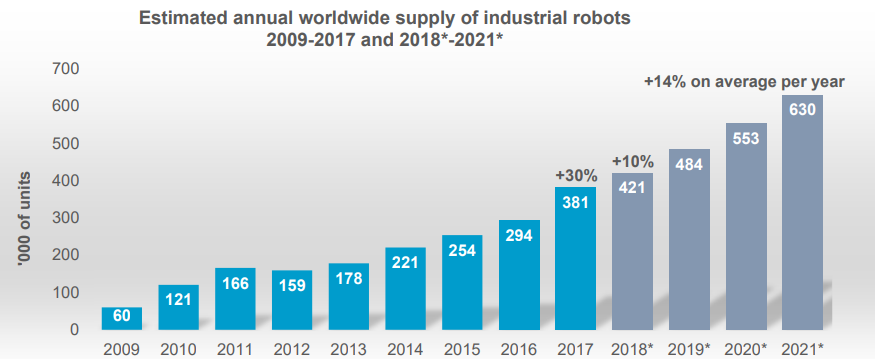
\includegraphics[width=0.5\textwidth]{just_1.PNG}
	\source{\cite{ifr2018}}		
\end{figure}

\begin{figure}[h!]										\caption{Demanda global de robôs em cada setor da indústria no período 2015-2017} \label{fig:just_2}		
	\centering										
	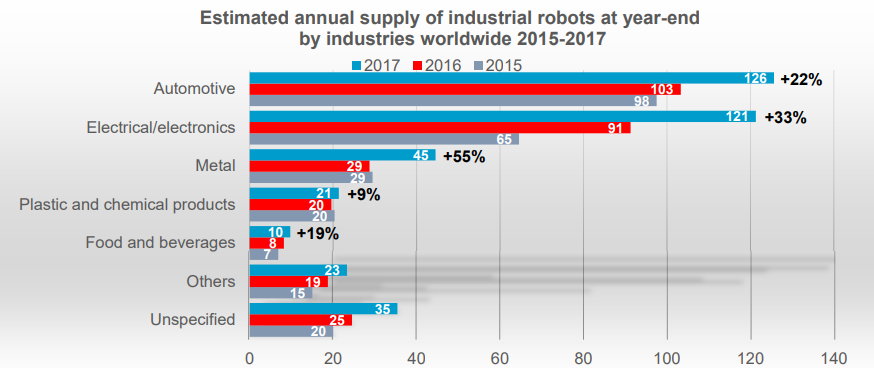
\includegraphics[width=0.5\textwidth]{just_2.PNG}
	\source{\cite{ifr2018}}		
\end{figure}

Esse aumento na demanda está presente em todas as áreas da indústria, como mostrado na figura ~\ref{fig:just_2}, com maior relevâncias nos setores eletroeletrônico e automotivo, de onde vêm as maiores expectativas de inovação por parte da população.
 
Um exemplo de tecnologia que está sendo desenvolvida nessa área, e que é uma das mais esperadas pelo público, são os carros autônomos, que prometem, além da condução independente, maior segurança para os passageiros e tomadas de decisões importantes como a escolha de rotas e ações para evitar acidentes.

Aliado a isso, existe um aumento na demanda por profissionais qualificados cada vez maior nesse setor. Em adição, há ainda uma notória dificuldade em capacitar trabalhadores para lidar com tecnologias as quais eles não tiveram contato durante o ensino médio e fundamental. Alguns conceitos, que não são novos, como sistemas autônomos, \textit{Machine Learning}, \textit{big data}, tem despertado a curiosidade e estimulando a imaginação da sociedade. Porém, isso vem trazendo alguns equívocos.

Um dos problemas encontrados na formação de profissionais para atuar na área da robótica, é que, diante destes “novos” conceitos as pessoas tendem a se retrair e ter uma noção equivocada, pensando que estes conceitos, que são primordiais para robótica, são extremamente difíceis e complexos, quando na verdade a abordagem de ensino não se preocupa com a desmistificação destes conceitos. É comum ouvir que a automação irá estabelecer novas relações trabalhistas, que irá extinguir alguns empregos e irá criar outros, porém, será que a nossa sociedade está preparada para estes novos empregos? 

Voltando ao campo da pedagogia, foi através de cenários semelhantes à este, que nasceram os movimentos Maker e STEM, oriundos da metodologia Do It Yourself (em português: faça você mesmo). Segundo \cite{Pugliese} ambos valorizam a possibilidade de utilizar das informações obtidas por pesquisa e conteúdo online de fácil acesso para fazer projetos com as próprias mãos. Esses projetos devem fomentar a utilização de equipamentos relacionados à áreas da ciência e da engenharia, seja com ajuda de um computador, impressora 3D ou ferramentas. Essa abordagem visa aumentar a atratividade para as áreas da ciência e desmistificar tabus relacionados à dificuldade de se aprender novas tecnologias.
 
Como resultado, mais jovens e adultos interessam-se por tecnologia, seguem carreiras na área e aumentam o número de profissionais qualificados no mercado.
Ainda no campo da pedagogia, segundo \cite{Mataric} o ensino da robótica é interdependente de aulas no formato da pedagogia clássica, porém melhor aproveitado quando associado a atividades práticas em grupo. Por este motivo considera-se que o movimento Maker e algumas metodologias de ensino de robótica são baseadas na concepção de Lev Vygotsky, onde o sujeito é considerado um ser não só ativo como também interativo, porque adquire conhecimentos a partir de relações intra e interpessoais, exercitando o que o homem tem de melhor: a criatividade.
 
Palangana, \cite{Palangana}, diz que segundo a concepção de Vygotsky, a aquisição de conhecimentos se dá pela interação do sujeito com o meio. Essa associação visa apresentar de forma menos abstrata conceitos abordados nas aulas teóricas e propor compartilhamento de aprendizagem e fomentar o trabalho em grupo entre os alunos dos níveis Fundamental II e Médio.

Analisando a conjuntura atual, uma nova abordagem ao ensino de conceitos básicos de robótica foi idealizada, sendo apresentada como um kit didático de robótica básica aplicada. Este kit terá como principal objetivo o ensino teórico e prático, de conceitos e ferramentas básicas utilizadas no mundo da robótica, em aplicações nos mais diversos setores da sociedade.
 
Tendo em vista o abordado acima, esta monografia tem como objetivo apresentar o projeto de um kit didático de aprendizagem de conceitos básicos em robótica aplicada, utilizando o framework ROS e aplicando conceitos básicos de cinemática e visão computacional.

%--------- NEW SECTION ----------------------
\section{Organização do \thetypework}
\label{section:organizacao}
O documento está organizado em cinco capítulos, seguindo a seguinte estrutura:

\textbf{Capitulo 1 - Introdução}: Faz a contextualização do âmbito no qual a pesquisa proposta
está inserida. Propõe justificar a problemática abordada, e porque a mesma é passível de uma solução. Apresenta, portanto, a problemática, as justificativas e os objetivos deste trabalho.


\textbf{Capítulo 2 - Referencial Teórico}: Apresenta o embasamento teórico que foi utilizado para melhor compor o desenvolvimento do projeto.

\textbf{Capítulo 3 - Metodologia}: Define as etapas de elaboração do trabalho, tal como as metodologias específicas utilizadas em cada etapa do desenvolvimento e suas justificativas.

\textbf{Capítulo 4 - Desenvolvimento}: Apresenta o que foi produzido neste trabalho do ponto de vista de todas as frentes abordadas, partindo das conclusões tiradas para iniciar as confecções dos tutoriais e do kit físico, até o resultado final das mesmas.

\textbf{Capítulo 5 - Conclusão}: Apresenta as conclusões tiradas acerca do que foi desenvolvido e das influências das metodologias utilizadas, tal como possíveis melhorias e expansões futuras.
